\documentclass{beamer}
%Для защит онлайн лучше использовать разрешение 16x9
%\documentclass[aspectratio=169]{beamer}

%%% Обязательные пакеты
%% Beamer
\usepackage{listings}

\usepackage{beamerthemesplit}
\usetheme{SPbGU}
\beamertemplatenavigationsymbolsempty
\usepackage{appendixnumberbeamer}

%% Локализация
\usepackage{fontspec}
\setmainfont{CMU Serif}
\setsansfont{CMU Sans Serif}
\setmonofont{CMU Typewriter Text}
%\setmonofont{Fira Code}[Contextuals=Alternate,Scale=0.9]
%\setmonofont{Inconsolata}
% \newfontfamily\cyrillicfont{CMU Serif}

\usepackage{polyglossia}
\setdefaultlanguage{russian}
\setotherlanguage{english}
\usepackage[autostyle]{csquotes} % Правильные кавычки в зависимости от языка

%% Графика
\usepackage{wrapfig} % Позволяет вставлять графику, обтекаемую текстом
\usepackage{pdfpages} % Позволяет вставлять многостраничные pdf документы в текст

%% Математика
\usepackage{amsmath, amsfonts, amssymb, amsthm, mathtools} % "Адекватная" работа с математикой в LaTeX

% Математические окружения с русским названием
\newtheorem{rutheorem}{Теорема}
\newtheorem{ruproof}{Доказательство}
\newtheorem{rudefinition}{Определение}
\newtheorem{rulemma}{Лемма}

%%% Дополнительные пакеты. Используются в презентации, но могут быть отключены при необходимости
\usepackage{tikz} % Мощный пакет для создание рисунков, однако может очень сильно замедлять компиляцию
\usetikzlibrary{decorations.pathreplacing,calc,shapes,positioning,tikzmark}

\usepackage{multirow} % Ячейка занимающая несколько строк в таблице

%% Пакеты для оформления алгоритмов на псевдокоде
\usepackage[noend]{algpseudocode}
\usepackage{algorithm}
\usepackage{algorithmicx}

\usepackage{fancyvrb}


% То, что в квадратных скобках, отображается внизу по центру каждого слайда.
\title[ACPI]{Advanced Configuration and Power Interface}

% То, что в квадратных скобках, отображается в левом нижнем углу.
\institute[]{}

% То, что в квадратных скобках, отображается в левом нижнем углу.
\author[Михайлов Илья]{Михайлов Илья}

\begin{document}
{
\setbeamertemplate{footline}{}
% Лого университета или организации, отображается в шапке титульного листа
\begin{frame}
	% \includegraphics[width=1.4cm]{pictures/SPbGU_Logo.png}
	\vspace{35pt}
	\hspace{-10pt}
	\begin{center}
		% \begin{tabular}{c}
		% 	\scriptsize{Санкт-Петербургский государственный университет} \\
		% 	\scriptsize{Кафедра системного программирования}
		% \end{tabular}
		\titlepage
	\end{center}

	\btVFill

	% {\scriptsize
	% 	% У научного руководителя должна быть указана научная степень
	% 	\textbf{Научный руководитель:} Косарев~Д.~С., ассистент кафедры системного программирования \\
	% 	% Консультанта может и не быть. Должна быть указана должность или ученая степень
	% 	% \textbf{Консультант:}  П.П. Петров, программист ЗАО \enquote{Компания с ну очень-очень-очень длинным названием}\\
	% 	% Для курсовой не обязателен. Должна быть указана должность или ученая степень
	% 	% \textbf{Рецензент:} д.т.н., проф. И.И. Иванов, исполнительный директор ООО \enquote{Рога и копыта}
	% }
	\begin{center}
		\vspace{5pt}
		\scriptsize{
			29.06.2024}
	\end{center}

\end{frame}
}

\begin{frame}
	\frametitle{Мотивация}
	\begin{itemize}
		\item Открытый промышленный стандарт, определяющий общий интерфейс
		\item Управление питанием, конфигурацией устройств и материнской платы со стороны ОС
		      % \item OS-directed motherboard configuration and power management
		\item Управление эффективностью энергопотребления и производительностью
		      % \item Introduction of laptops and problem of battery efficeincy
		\item Auto configuration (Hot plugging \& Hot swapping)
	\end{itemize}
\end{frame}

\begin{frame}
	\frametitle{История}
	\begin{itemize}
		\item Декабрь 1996-го года -- первая публикация
		\item Сентябрь 2004-го года -- версия 3.0; поддержка SATA, PCE-E; многоядерность
		\item Июнь 2009-го года -- версия 4.0; поддержка USB 3.0, x2APIC
		\item Август 2022-го года -- последняя версия 6.5
	\end{itemize}
	\hspace{86pt}
	
\includegraphics[width=160pt]{pictures/trouble2.jpg}
\end{frame}

\begin{frame}
	\frametitle{Архитектура}
	\begin{itemize}
		\item Спецификация --> Исходный код ASL --> Байткод AML --> Firmware
		\item Во время загрузки ОС интерпретатор байткода генерирует ACPI namespace из таблиц
		\item ACPI namespace -- древообразная структура
		\item Интерпретатор и ACPI namespace находятся в пространстве ядра
	\end{itemize}
\end{frame}

\begin{frame}
	\frametitle{Архитектура}
	\hspace{18pt}
	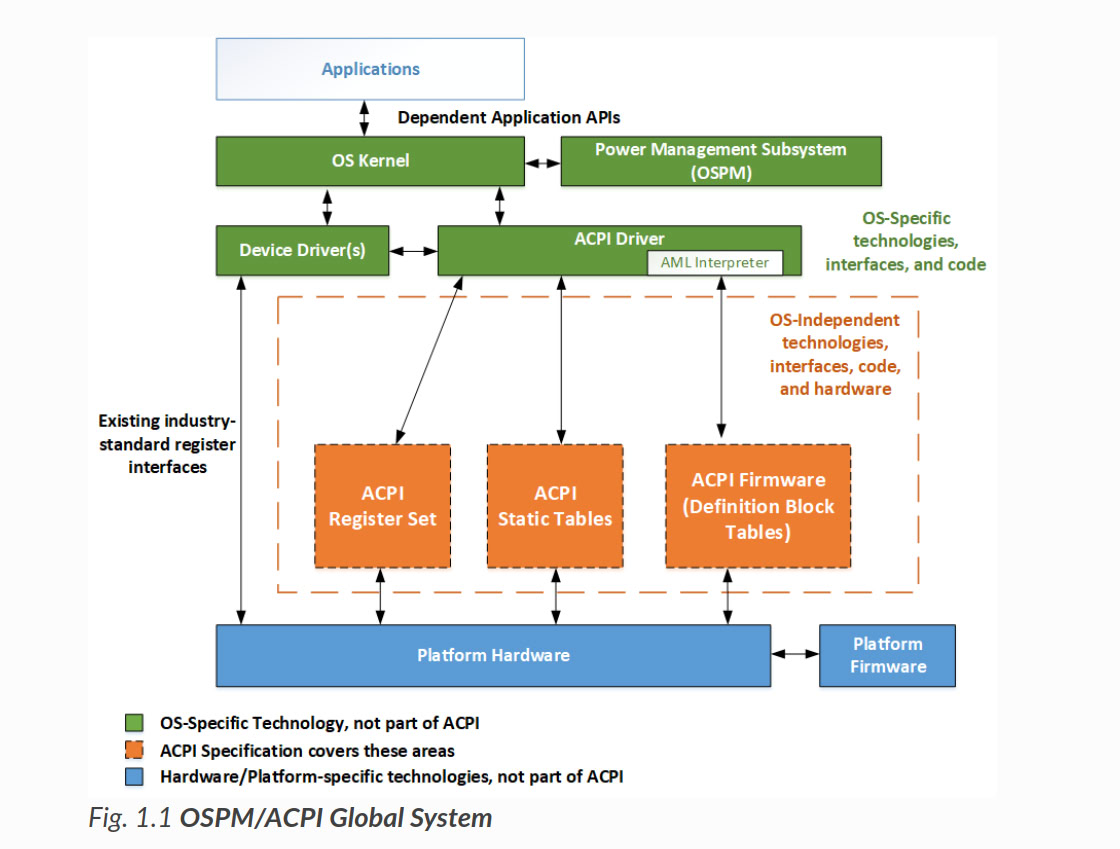
\includegraphics[width=300pt]{pictures/arch_acpi1.jpg}
\end{frame}

\begin{frame}
	\frametitle{Power States}
	\hspace{18pt}
	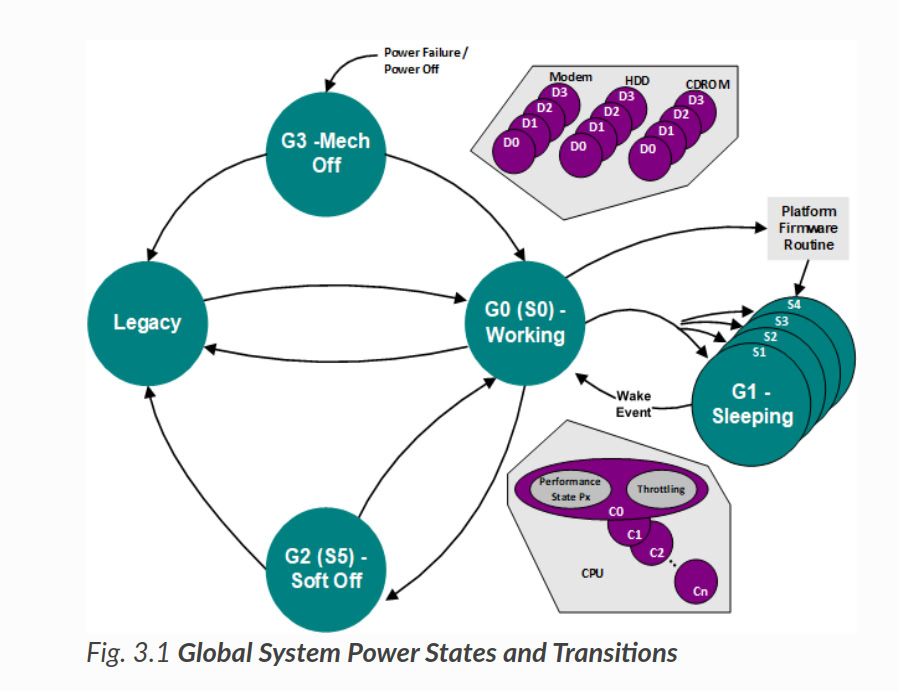
\includegraphics[width=300pt]{pictures/arch_acpi2.jpg}
\end{frame}

\begin{frame}
	\frametitle{Таблицы}
	\hspace{18pt}
	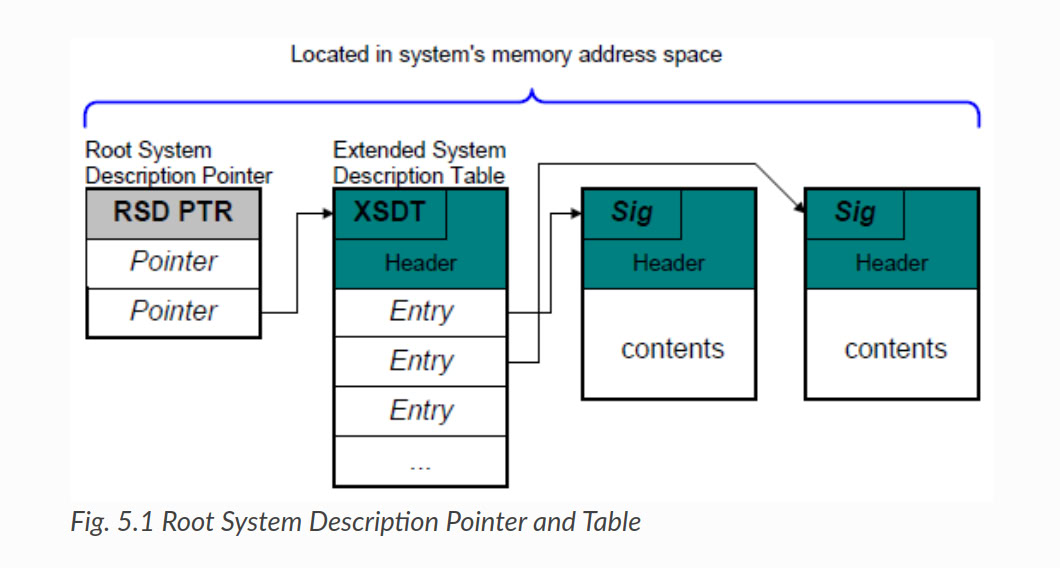
\includegraphics[width=300pt]{pictures/arch3.jpg}
\end{frame}

\begin{frame}
	\frametitle{Таблицы}
	\hspace{18pt}
	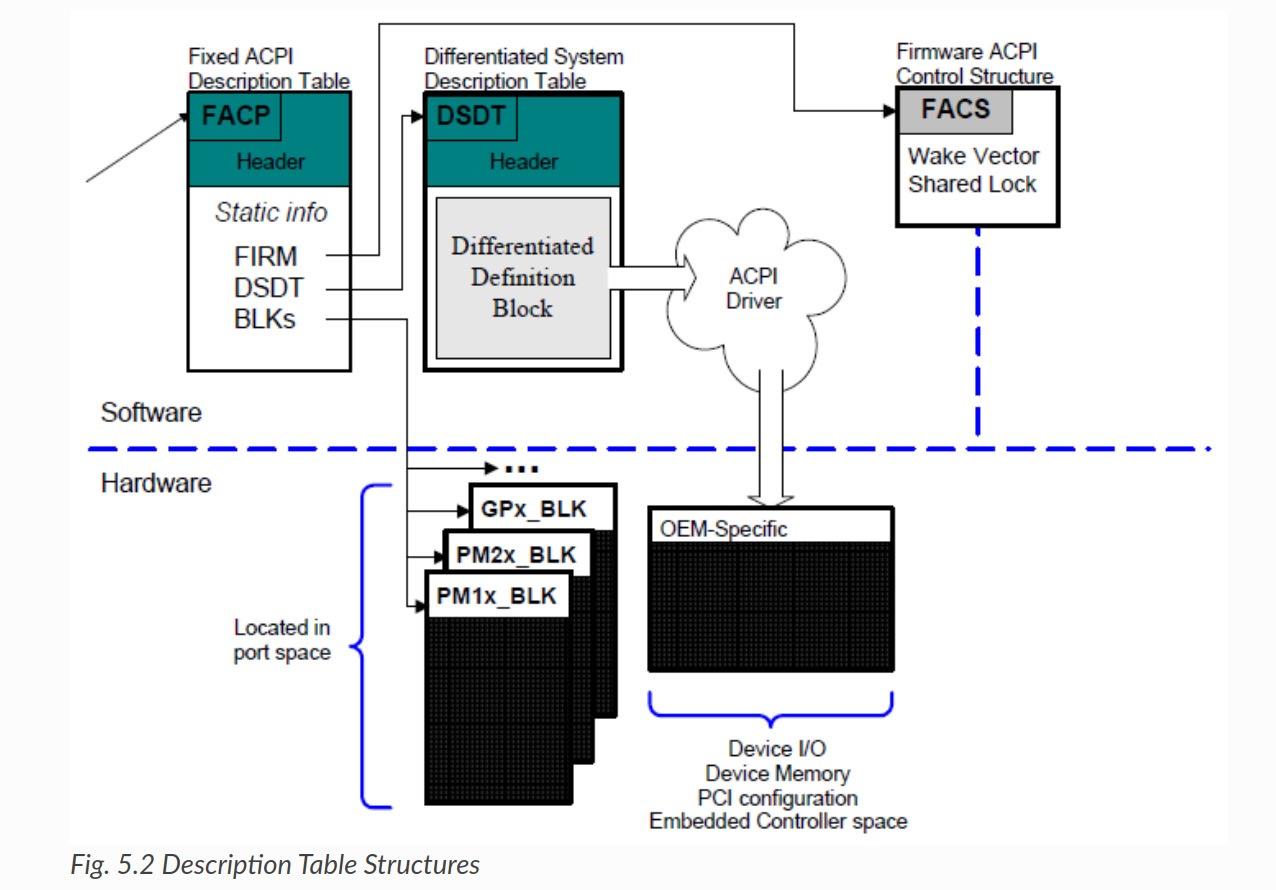
\includegraphics[width=300pt]{pictures/arch4.jpg}
\end{frame}

% \begin{frame}
% 	\frametitle{Как программировать}
% \end{frame}

\begin{frame}
	\frametitle{Критика}
	\hspace{18pt}
	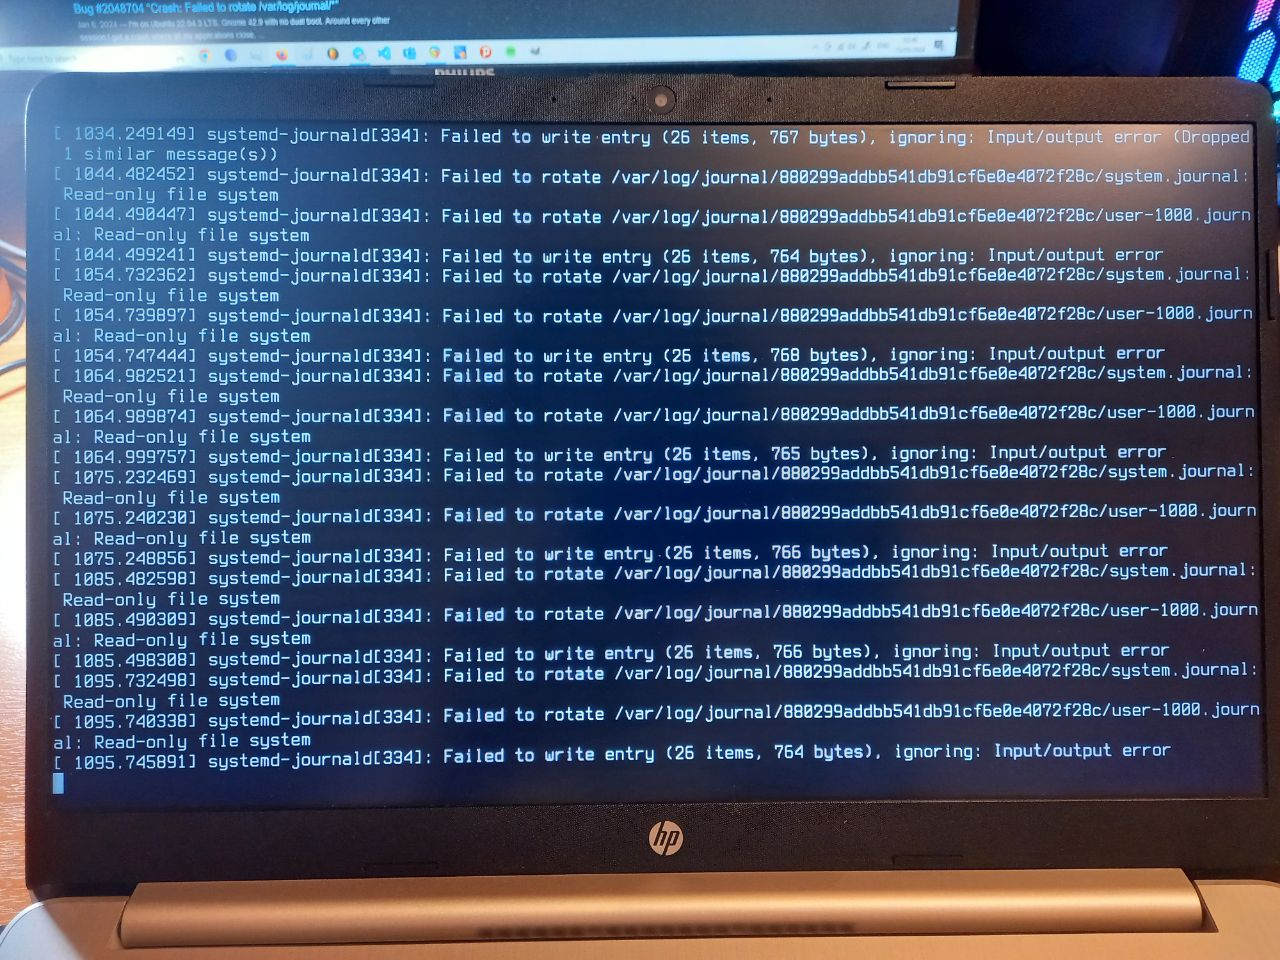
\includegraphics[width=300pt]{pictures/trouble1.jpg}
\end{frame}

\begin{frame}
	\frametitle{Источники}
	\begin{itemize}
		\item \href{https://uefi.org/htmlspecs/ACPI\_Spec\_6\_4\_html/}{https://uefi.org/htmlspecs/ACPI\_Spec\_6\_4\_html/}
		\item \href{https://en.wikipedia.org/wiki/ACPI}{https://en.wikipedia.org/wiki/ACPI}
		\item \href{https://www.google.com/url?sa=t\&source=web\&rct=j\&opi=89978449\&url=https://cdrdv2-public.intel.com/772722/asl-tutorial-v20190625.pdf\&ved=2ahUKEwiDuOfEqoCHAxWiLBAIHcLiDJkQFnoECB4QAQ\&usg=AOvVaw3oEVdOF0XZO01rL0uN\_9go}{https://www.google.com/url?sa=t\&source=web\&rct=j\&opi=89978449\&url=https://cdrdv2-public.intel.com/772722/asl-tutorial-v20190625.pdf\&ved=2ahUKEwiDuOfEqoCHAxWiLBAIHcLiDJkQFnoECB4QAQ\&usg=AOvVaw3oEVdOF0XZO01rL0uN\_9go}
		\item \href{https://youtu.be/nlKjUAv3RL0?si=Z1CC0ofQXbPK9vSa}{https://youtu.be/nlKjUAv3RL0?si=Z1CC0ofQXbPK9vSa}
	\end{itemize}
\end{frame}

% \begin{frame}[fragile]
% 	\frametitle{Введение}
% 	\begin{itemize}
% 		% \item Краткий обзор тематики работы (как вариант~--- устно, пока показывается титульный слайд)
% 		% \item Не нужно определять общеизвестные понятия
% 		% \item Применимость/полезность данной работы, обоснование выбора именно этой темы
% 		% \item Если тема похожа на темы других работ (в том числе прошлых лет), надо явно описать разницу
% 		\item Системы сборки --- неотъемлемая часть автоматизации разработки ПО
% 		\item Mybuild --- система сборки конфигурируемой ОСРВ Embox
% 		\item Реализация Mybuild написана на GNU Make
% 		\item Предлагается написать реализацию на высокоуровневом функциональном языке OCaml
% 	\end{itemize}
% \end{frame}

% \begin{frame}
% 	\frametitle{Существующие решения}
% 	\begin{itemize}
% 		% \item Перечислить инструменты/подходы, применяемые в области
% 		% \item Указать их преимущества и недостатки (критика существующих решений/подходов)
% 		\item GNU Make
% 		\item Kbuild \footnote{\href{https://docs.kernel.org/kbuild/index.html}{https://docs.kernel.org/kbuild/index.html}}
% 		\item Системы сборки использующие другие билд-системы, как бэкэнд \begin{itemize}
% 			      \item СMake, Meson \footnote{\href{https://mesonbuild.com/}{https://mesonbuild.com/}}
% 		      \end{itemize}
% 		\item Dune, Ninja
% 	\end{itemize}

% \end{frame}

% % \begin{frame}
% % 	\frametitle{Существующие решения}
% % 	Возможно, предметная область сложна и потребуется больше одного слайда, но затягивать введение не стоит. Постарайтесь уложиться в 1--2 слайда
% % 	\begin{itemize}
% % 		\item Выводы
% % 		      \begin{itemize}
% % 			      \item Подвести итог
% % 			      \item Указать недостатки существующих подходов, на борьбу с которыми
% % 			            направленна данная работа
% % 			      \item Чётко сформулировать существующую проблему, которая будет решаться в данной работе
% % 		      \end{itemize}
% % 	\end{itemize}
% % \end{frame}

% % Обязательный слайд: четкая формулировка цели данной работы и постановка задачи
% % Описание выносимых на защиту результатов, процесса или особенностей их достижения и т.д.
% \begin{frame}
% 	\frametitle{Постановка задачи}
% 	\textbf{Целью} работы является реинжиниринг системы сборки Mybuild.

% 	\textbf{Задачи} на осенний семестр:
% 	\begin{itemize}
% 		\item Реализовать парсер декларативного языка Myfile %основываясь на проведённом анализе проблемы, области, существующих решений
% 		\item Протестировать парсер языка Myfile на существующей кодовой базе
% 	\end{itemize}
% \end{frame}

% %Идеально, если есть по одному слайду на каждую поставленную задачу

% \begin{frame}
% 	\frametitle{Обзор Mybuild (1/4)}
% 	\begin{itemize}
% 		\item Система сборки написана на синтаксическом расширении GNU Make
% 		\item Генерирует конкретный образ ОС по описаниям модулей и конфигурации
% 		\item 	Процесс сборки состоит из:
% 		      \begin{itemize}
% 			      \item подготовки скриптов
% 			      \item создания графа описания модулей
% 			      \item создания модели системы
% 			      \item генерации необходимых ресурсов
% 			      \item запуска скриптов на исполнение
% 		      \end{itemize}
% 	\end{itemize}
% \end{frame}

% \begin{frame}
% 	\frametitle{Обзор Mybuild (2/4)}
% 	В Mybuild реализовано два декларативных языка программирования:
% 	\begin{itemize}
% 		\item Myfile — для описания модулей
% 		\item Configfile — для описания конфигураций
% 	\end{itemize}
% 	В качестве инструмента для синтаксического анализа используется генератор LALR-парсеров GOLD \footnote{\href{http://www.goldparser.org/}{http://www.goldparser.org/}}
% \end{frame}

% \begin{frame}
% 	\frametitle{Обзор Mybuild (3/4)}
% 	Для каждого модуля в Build-модели необходимо:
% 	\begin{itemize}
% 		\item Включить сам модуль
% 		\item Включить все его зависимости и провести проверку (например, включить реализацию по-умолчанию для абстрактного модуля, если никакой другой реализации не было включено)
% 		\item Сопоставить значениям аргументов, указанных в конфигурационных файлах, значения опций модуля
% 	\end{itemize}
% \end{frame}

% \begin{frame}
% 	\frametitle{Обзор Mybuild (4/4)}
% 	За генерацию необходимых ресурсов отвечает скрипт build-gen.mk, который порождает:
% 	\begin{itemize}
% 		\item Исходные файлы на языке C, содержащие run-time представление Build-модели
% 		\item Заголовочные файлы с необходимыми опциями; также происходит копирование исходных заголовочных файлов модуля
% 		      % \item командные файлы для файлов с исходным кодом, содержащие параметры командной строки компилятора;
% 		\item Make-файлы c правилами для сборки целевого образа и промежуточных объектных файлов
% 	\end{itemize}
% \end{frame}

% % \begin{frame}[fragile]
% % 	\frametitle{Новый алгоритм\footnote{Иллюстративные возможности: таблицы, картинки, код}}
% % 	% Задается ширина столбцов
% % 	\begin{tabular}{p{5cm} p{7cm}}
% % 		% Фрагмент кода
% % 		\begin{minipage}{3in}
% % 			\begin{Verbatim}[commandchars=\\\{\}]

% % 				\textcolor{blue}{string} res = \textcolor{orange}{""};
% % 				\textcolor{blue}{for}(i = 0; i < l; i++) \{
% % 				res = \textcolor{orange}{"()"} + res;
% % 				\}

% % 			\end{Verbatim}
% % 		\end{minipage}
% % 		&
% % 		Результат (SPPF):
% % 		\\
% % 		Аппроксимация:
% % 		&
% % 		% Картинка. Изображения должны быть векторными. Исключения --- снимки экрана.
% % 		\multirow{-2}*{\!\includegraphics[width=6.8cm]{pictures/out3.pdf}}
% % 		\\
% % 		\includegraphics[width=2.5cm]{pictures/in3.pdf}
% % 		&
% % 		\\
% % 		Грамматика: &
% % 		\\
% % 		\vspace{-20pt}
% % 		% Можно формулы писать
% % 		{\begin{align*}
% % 				start& & &\Coloneq & &s \\
% % 				s & & &\Coloneq & &\mbox{\texttt{LBR }} s \mbox{\texttt{ RBR }} s \\
% % 				s & & &\Coloneq & &\epsilon
% % 			\end{align*}}
% % 		&
% % 	\end{tabular}
% % \end{frame}

% % \begin{frame}[fragile]
% % 	\frametitle{Доказательство корректности алгоритма}
% % 	{\tiny Формулировки утверждений. Идеи доказательств проговариваются устно.}
% % 	\begin{rutheorem}[Пифагора: геометрическая формулировка]
% % 		В прямоугольном треугольнике площадь квадрата, построенного на гипотенузе, равна сумме площадей квадратов, построенных на катетах.
% % 	\end{rutheorem}

% % 	\begin{rutheorem}[Пифагора: алгебраическая формулировка]
% % 		В прямоугольном треугольнике квадрат длины гипотенузы равен сумме квадратов длин катетов.

% % 		То есть, если обозначить длину гипотенузы треугольника через $c$, а длины катетов
% % 		через $a$ и $b$, получим верное равенство: $a^2 + b^2 = c^2$.
% % 	\end{rutheorem}

% % 	\begin{rutheorem}[Обратная теорема Пифагора]
% % 		Для всякой тройки положительных чисел $a$, $b$ и $c$, такой, что $a^2 + b^2 = c^2$, существует прямоугольный треугольник с катетами $a$ и $b$ и гипотенузой $c$.
% % 	\end{rutheorem}
% % \end{frame}

% \begin{frame}[fragile]
% 	\frametitle{Реализация (1/2)}
% 	\begin{itemize}
% 		\item Спроектирована структуры данных для АСТ
% 		\item Menhir был использован для синтаксического анализа
% 		\item ocamllex был использован лексического анализа
% 	\end{itemize}
% \end{frame}

% \begin{frame}[fragile]
% 	\frametitle{Реализация (2/2)}
% 	\begin{lstlisting}[language=caml, frame=single, breaklines, basicstyle=\footnotesize]
%   $ dune exec ../../src/parser/parse.exe /home/cy/Desktop/ocaml-rep/embox/src/mem/Mybuild
%   ((Some ["embox"; "mem"]), [],
%    [([],
%      (Module
%         ([], "phymem", None,
%          [([], (Opt (NumberType, "log_level", (Some (NumberLiteral 3.)))));
%            ([], (Source ["phymem.c"]));
%            ([], (Depends [["embox"; "mem"; "vmem_device_memory"]]));
%            ([], (Depends [["embox"; "mem"; "sections"]]))])))
%      ])
%   \end{lstlisting}
% \end{frame}

% \begin{frame}
% 	\frametitle{Тестирование}
% 	\begin{itemize}
% 		\item Парсер был протестирован на файлах Mybuild из репозитория Embox, используя cram-тесты \footnote{\href{https://github.com/mikhaylovilya/caravan/blob/master/test/parser\_test/parse\_myfiles.t}{https://github.com/mikhaylovilya/caravan/blob/master/test/parser\_test/parse\_myfiles.t} (дата обращения: 08.01.2024)}
% 		\item С помощью Github Actions была реализована непрерывная интеграция, где происходит сборка проекта при помощи dune, а также запуск тестов.
% 	\end{itemize}
% \end{frame}

% \begin{frame}
% 	\frametitle{Результаты}
% 	В результате проведенной работы были выполнены следующие задачи:
% 	\begin{enumerate}
% 		\item Написана реализация парсера декларативного языка Myfile
% 		\item Проведено тестирование парсера на существующей кодовой базе в репозитории Embox
% 	\end{enumerate}

% 	Исходный код работы доступен по ссылке \footnote{\href{https://github.com/mikhaylovilya/caravan}{https://github.com/mikhaylovilya/caravan} (дата обращения: 08.01.2024)}.
% 	Имя аккаунта: mikhaylovilya. Название репозитория: caravan.
% \end{frame}

%\addtocounter{framenumber}{1}
\appendix

\end{document}
